\documentclass[tikz,border=4pt]{standalone}

\usepackage[T1]{fontenc}
\renewcommand{\rmdefault}{ptm}
\usetikzlibrary{arrows.meta,positioning}

% Palette shared with the main publication figure and Figure 5.
\definecolor{Ink}{HTML}{1D303C}
\definecolor{FlowInk}{HTML}{526570}
\definecolor{DataColor}{HTML}{2B6F8A}
\definecolor{ProcessColor}{HTML}{6B5A94}
\definecolor{RecoveryColor}{HTML}{B56A24}
\definecolor{EvaluationColor}{HTML}{337A58}

\tikzset{
  outer flow/.style={-{Latex[length=1.8mm,width=1.25mm]}, draw=FlowInk, line width=0.8pt},
  data flow/.style={-{Latex[length=1.55mm,width=1.05mm]}, draw=DataColor, line width=0.75pt},
  process flow/.style={-{Latex[length=1.55mm,width=1.05mm]}, draw=ProcessColor, line width=0.75pt},
  recovery flow/.style={-{Latex[length=1.55mm,width=1.05mm]}, draw=RecoveryColor, line width=0.75pt},
  evaluation flow/.style={-{Latex[length=1.55mm,width=1.05mm]}, draw=EvaluationColor, line width=0.75pt},
  data group/.style={draw=DataColor!42!white,
    top color=DataColor!18!white, bottom color=DataColor!5!white,
    rounded corners=4.0pt, line width=0.8pt},
  process group/.style={draw=ProcessColor!42!white,
    top color=ProcessColor!18!white, bottom color=ProcessColor!5!white,
    rounded corners=4.0pt, line width=0.8pt},
  recovery group/.style={draw=RecoveryColor!42!white,
    top color=RecoveryColor!18!white, bottom color=RecoveryColor!5!white,
    rounded corners=4.0pt, line width=0.8pt},
  evaluation group/.style={draw=EvaluationColor!42!white,
    top color=EvaluationColor!18!white, bottom color=EvaluationColor!5!white,
    rounded corners=4.0pt, line width=0.8pt},
  data step/.style={draw=DataColor!30!white, fill=DataColor!5!white,
    rounded corners=2.0pt, line width=0.65pt, align=center, text=Ink,
    font=\rmfamily\fontsize{7.2}{8.3}\selectfont, inner sep=2.0pt},
  process step/.style={draw=ProcessColor!30!white, fill=ProcessColor!5!white,
    rounded corners=2.0pt, line width=0.65pt, align=center, text=Ink,
    font=\rmfamily\fontsize{7.2}{8.3}\selectfont, inner sep=2.0pt},
  recovery step/.style={draw=RecoveryColor!30!white, fill=RecoveryColor!5!white,
    rounded corners=2.0pt, line width=0.65pt, align=center, text=Ink,
    font=\rmfamily\fontsize{7.2}{8.3}\selectfont, inner sep=2.0pt},
  evaluation step/.style={draw=EvaluationColor!30!white, fill=EvaluationColor!5!white,
    rounded corners=2.0pt, line width=0.65pt, align=center, text=Ink,
    font=\rmfamily\fontsize{7.2}{8.3}\selectfont, inner sep=2.0pt},
  stage title/.style={font=\rmfamily\bfseries\fontsize{7.8}{8.8}\selectfont, align=center},
}

\newcommand{\stagegap}{3.0mm}

\begin{document}
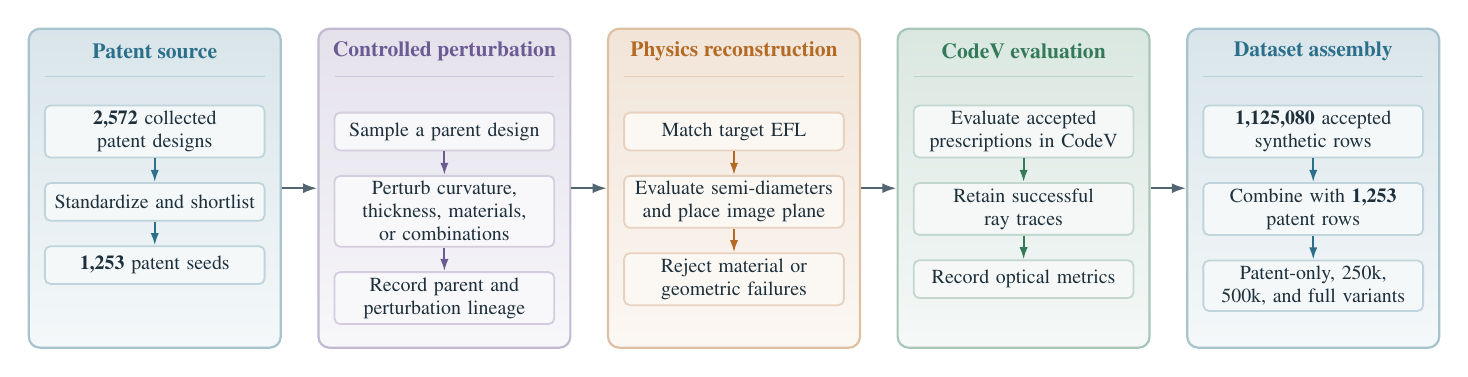
\begin{tikzpicture}[node distance=4.5mm]
  % Five equal stages keep the construction sequence compact and comparable.
  \node[data group, minimum width=3.20cm, minimum height=4.05cm] (source) {};
  \node[process group, minimum width=3.20cm, minimum height=4.05cm, right=of source] (perturb) {};
  \node[recovery group, minimum width=3.20cm, minimum height=4.05cm, right=of perturb] (reconstruct) {};
  \node[evaluation group, minimum width=3.20cm, minimum height=4.05cm, right=of reconstruct] (simulate) {};
  \node[data group, minimum width=3.20cm, minimum height=4.05cm, right=of simulate] (assemble) {};

  \node[stage title, text=DataColor] at ([yshift=-3.0mm]source.north) {Patent source};
  \node[stage title, text=ProcessColor] at ([yshift=-3.0mm]perturb.north) {Controlled perturbation};
  \node[stage title, text=RecoveryColor] at ([yshift=-3.0mm]reconstruct.north) {Physics reconstruction};
  \node[stage title, text=EvaluationColor] at ([yshift=-3.0mm]simulate.north) {CodeV evaluation};
  \node[stage title, text=DataColor] at ([yshift=-3.0mm]assemble.north) {Dataset assembly};

  % Header rules echo the main publication figure.
  \draw[DataColor!34!white, line width=0.45pt]
    ([xshift=2.2mm,yshift=-6.2mm]source.north west) --
    ([xshift=-2.2mm,yshift=-6.2mm]source.north east);
  \draw[ProcessColor!34!white, line width=0.45pt]
    ([xshift=2.2mm,yshift=-6.2mm]perturb.north west) --
    ([xshift=-2.2mm,yshift=-6.2mm]perturb.north east);
  \draw[RecoveryColor!34!white, line width=0.45pt]
    ([xshift=2.2mm,yshift=-6.2mm]reconstruct.north west) --
    ([xshift=-2.2mm,yshift=-6.2mm]reconstruct.north east);
  \draw[EvaluationColor!34!white, line width=0.45pt]
    ([xshift=2.2mm,yshift=-6.2mm]simulate.north west) --
    ([xshift=-2.2mm,yshift=-6.2mm]simulate.north east);
  \draw[DataColor!34!white, line width=0.45pt]
    ([xshift=2.2mm,yshift=-6.2mm]assemble.north west) --
    ([xshift=-2.2mm,yshift=-6.2mm]assemble.north east);

  % Patent source.
  \node[data step, text width=2.65cm, minimum height=0.48cm] (collected)
    at ([yshift=7.2mm]source.center) {\textbf{2,572} collected\\patent designs};
  \node[data step, text width=2.65cm, minimum height=0.48cm, below=\stagegap of collected] (standardize)
    {Standardize and shortlist};
  \node[data step, text width=2.65cm, minimum height=0.48cm, below=\stagegap of standardize] (seeds)
    {\textbf{1,253} patent seeds};

  % Controlled perturbation.
  \node[process step, text width=2.65cm, minimum height=0.48cm] (parent)
    at ([yshift=7.2mm]perturb.center) {Sample a parent design};
  \node[process step, text width=2.65cm, minimum height=0.48cm, below=\stagegap of parent] (variants)
    {Perturb curvature,\\thickness, materials,\\or combinations};
  \node[process step, text width=2.65cm, minimum height=0.48cm, below=\stagegap of variants] (lineage)
    {Record parent and\\perturbation lineage};

  % Physics reconstruction and validity gate.
  \node[recovery step, text width=2.65cm, minimum height=0.48cm] (efl)
    at ([yshift=7.2mm]reconstruct.center) {Match target EFL};
  \node[recovery step, text width=2.65cm, minimum height=0.48cm, below=\stagegap of efl] (geometry)
    {Evaluate semi-diameters\\and place image plane};
  \node[recovery step, text width=2.65cm, minimum height=0.48cm, below=\stagegap of geometry] (reject)
    {Reject material or\\geometric failures};

  % Simulation validation and optical annotation.
  \node[evaluation step, text width=2.65cm, minimum height=0.48cm] (codev)
    at ([yshift=7.2mm]simulate.center) {Evaluate accepted\\prescriptions in CodeV};
  \node[evaluation step, text width=2.65cm, minimum height=0.48cm, below=\stagegap of codev] (traces)
    {Retain successful\\ray traces};
  \node[evaluation step, text width=2.65cm, minimum height=0.48cm, below=\stagegap of traces] (metrics)
    {Record optical metrics};

  % Final traceable dataset and study variants.
  \node[data step, text width=2.65cm, minimum height=0.48cm] (synthetic)
    at ([yshift=7.2mm]assemble.center) {\textbf{1,125,080} accepted\\synthetic rows};
  \node[data step, text width=2.65cm, minimum height=0.48cm, below=\stagegap of synthetic] (combined)
    {Combine with \textbf{1,253}\\patent rows};
  \node[data step, text width=2.65cm, minimum height=0.48cm, below=\stagegap of combined] (variantsOut)
    {Patent-only, 250k,\\500k, and full variants};

  % Within-stage flow.
  \draw[data flow] (collected.south) -- (standardize.north);
  \draw[data flow] (standardize.south) -- (seeds.north);
  \draw[process flow] (parent.south) -- (variants.north);
  \draw[process flow] (variants.south) -- (lineage.north);
  \draw[recovery flow] (efl.south) -- (geometry.north);
  \draw[recovery flow] (geometry.south) -- (reject.north);
  \draw[evaluation flow] (codev.south) -- (traces.north);
  \draw[evaluation flow] (traces.south) -- (metrics.north);
  \draw[data flow] (synthetic.south) -- (combined.north);
  \draw[data flow] (combined.south) -- (variantsOut.north);

  % Stage-to-stage flow.
  \draw[outer flow] (source.east) -- (perturb.west);
  \draw[outer flow] (perturb.east) -- (reconstruct.west);
  \draw[outer flow] (reconstruct.east) -- (simulate.west);
  \draw[outer flow] (simulate.east) -- (assemble.west);
\end{tikzpicture}
\end{document}
